% =====================================================================
%  Producto de difusión — Proyecto Integrador
%  Clasificación morfológica de galaxias usando espectros e imágenes
%  NOTA: si su curso proporciona una plantilla LaTeX oficial, copie el
%  cuerpo (desde \begin{abstract}) dentro de dicha plantilla.
% =====================================================================
\documentclass[11pt,a4paper]{article}
\usepackage[utf8]{inputenc}
\usepackage[T1]{fontenc}
\usepackage{lmodern}
\IfFileExists{spanish.ldf}{\usepackage[spanish,es-tabla,es-nodecimaldot]{babel}}{\usepackage[english]{babel}}
\usepackage[margin=2.5cm]{geometry}
\usepackage{amsmath,amssymb}
\usepackage{graphicx}
\usepackage{booktabs}
\usepackage{tabularx}
\usepackage{xcolor}
\usepackage{microtype}
\usepackage{fancyhdr}
\usepackage[round,authoryear]{natbib}
\usepackage[colorlinks=true,linkcolor=teal,citecolor=teal,urlcolor=teal]{hyperref}

% Nombres en español (funciona con o sin babel-spanish)
\renewcommand{\figurename}{Figura}
\renewcommand{\tablename}{Tabla}
\renewcommand{\refname}{Referencias}
\renewcommand{\abstractname}{Resumen}
\renewcommand{\contentsname}{Contenido}
\renewcommand{\appendixname}{Anexo}

\pagestyle{fancy}
\fancyhf{}
\fancyhead[L]{\small Clasificación morfológica de galaxias usando espectros e imágenes}
\fancyhead[R]{\small Proyecto Integrador}
\fancyfoot[C]{\thepage}
\setlength{\headheight}{14pt}
\newcolumntype{Y}{>{\raggedright\arraybackslash}X}
\setlength{\parskip}{3pt}

\title{\textbf{Clasificación morfológica de galaxias usando espectros e imágenes:\\ de la hipótesis multimodal a un clasificador visual verificable}}
\author{[Nombre(s) del equipo] \\ \small Proyecto Integrador · Producto de difusión}
\date{Noviembre de 2026}

\begin{document}
\maketitle
\thispagestyle{fancy}

% =====================================================================
\begin{abstract}
\noindent
La clasificación morfológica de galaxias en tempranas (elípticas y lenticulares) y tardías (espirales e irregulares) sigue dependiendo de la inspección visual, un proceso lento y subjetivo que no escala a los catálogos del Observatorio Vera C.\ Rubin (LSST). Este trabajo evaluó si combinar imágenes ópticas del Legacy Survey con espectros integrados de MaNGA y productos de síntesis de poblaciones estelares de STARLIGHT mejora la clasificación binaria frente a una sola modalidad. Con una cohorte alineada de 9,351 galaxias y una partición estratificada única (6,545/1,403/1,403), se construyó una línea base visual (ResNet-18; ROC-AUC = 0.9633, exactitud = 88.8\,\%) y se compararon encoders espectrales, de poblaciones y fusiones por concatenación bajo el mismo protocolo. La imagen dominó: el mejor modelo, una CNN visual entrenada con tasa de aprendizaje $3\times10^{-4}$, alcanzó ROC-AUC = 0.9667 y exactitud = 89.5\,\%, superando el umbral de aceptación (AUC $\geq 0.95$) por 0.0167, con un incremento de +0.0034 sobre la línea base, inferior a la incertidumbre estimada del AUC ($\approx 0.005$). Ninguna fusión mejoró de forma estadísticamente demostrable (fusión tardía: $\Delta$AUC = +0.0005, IC\,95\,\% $[-0.0012,\,+0.0022]$). Sin embargo, los errores no son idénticos: el experto de poblaciones acierta 51.6\,\% de los errores visuales, y el 47.8\,\% de esos errores se concentra en la frontera Ttype 0–1, donde la etiqueta humana es más ambigua. Se recomienda operar el clasificador visual con calibración y revisión experta en la zona incierta, y se plantea como trabajo futuro un decisor adaptativo por galaxia.

\medskip
\noindent\textbf{Palabras clave:} morfología galáctica, aprendizaje profundo, multimodalidad, MaNGA, Legacy Survey, CRISP-ML(Q).
\end{abstract}

\tableofcontents
\newpage

% =====================================================================
\section{Contexto de negocio y problema}
\label{sec:contexto}

\subsection{El problema científico como problema de ``negocio''}
La división entre galaxias tempranas (ETG) y tardías (LTG) es la partición de primer orden de la secuencia de Hubble y el punto de partida de casi cualquier estudio estadístico de poblaciones galácticas \citep{hubble1926,buta2013}. Históricamente se ha resuelto mediante inspección visual por especialistas: un proceso costoso, poco reproducible y con dispersión apreciable entre clasificadores independientes, sobre todo en los tipos intermedios. Los catálogos visuales que sustentan este proyecto \citep{nair2010,vazquezmata2022} muestran a la vez el valor y el costo humano de este enfoque. La llegada de LSST \citep{ivezic2019}, con miles de millones de galaxias, vuelve inviable la clasificación manual y convierte la automatización en una necesidad operativa.

En términos de CRISP-ML(Q) \citep{studer2021}, el ``cliente'' es la comunidad astronómica que explota catálogos; el producto es una probabilidad $P(\text{tardía})$ por galaxia, fiable, reproducible y escalable; y el valor se mide en tres niveles: científico (clasificación confiable), de aprendizaje automático (métricas en prueba ciega) y económico (costo y cobertura frente a la revisión humana).

\subsection{Planteamiento original (Avance 0)}
El planteamiento inicial formuló una hipótesis de complementariedad: la imagen codifica la \emph{forma} (concentración de luz, disco, brazos, barras) y el espectro la \emph{física} (edad de las poblaciones estelares, quiebre de 4000\,\AA, líneas de emisión ligadas a formación estelar). Por ello se esperaba que un modelo que combinara imagen y espectro superara a cualquier modalidad aislada. La etiqueta binaria se definió a partir de Ttype: temprana si $\text{Ttype}\leq 0$ y tardía si $1\leq\text{Ttype}\leq 10$. El alcance comprendió las fases 1 a 4 de CRISP-ML(Q); el despliegue y el monitoreo quedaron fuera de alcance, aunque sus requisitos se anticipan en la Sección~\ref{sec:implementacion}.

\subsection{Criterios de éxito acordados}
La Tabla~\ref{tab:criterios} resume los umbrales propuestos en la fase de entendimiento del negocio. Son el patrón contra el que se juzga el resultado en la Sección~\ref{sec:resultados}.

\begin{table}[htbp]
\centering
\caption{Criterios de éxito del proyecto (propuesta de la fase 1 de CRISP-ML(Q)).}
\label{tab:criterios}
\small
\begin{tabularx}{\textwidth}{lYY}
\toprule
\textbf{Nivel} & \textbf{Criterio} & \textbf{Cómo se mide}\\
\midrule
Científico & Clasificación ETG/LTG fiable y reproducible; demostrar que imagen + espectro supera a la mejor modalidad individual & Informe revisado por experto de dominio\\
ML (mínimo aceptable) & ROC-AUC $\geq 0.95$; exactitud balanceada $\geq 0.90$; ECE $\leq 0.05$; mejora multimodal con IC\,95\,\% que excluya 0 & Prueba ciega; bootstrap; McNemar\\
Económico & Costo por galaxia; galaxias por hora-GPU; cobertura con precisión $\geq 95\,\%$ (el resto a revisión humana) & Registro de tiempos; curva cobertura-precisión\\
\bottomrule
\end{tabularx}
\end{table}

\subsection{Cambio de enfoque: el enfoque finalmente adoptado}
El proyecto modificó su enfoque en tres puntos, todos documentados durante los avances:
\begin{enumerate}
  \item \textbf{Espectro de referencia.} El Avance 0 proponía iniciar con el espectro a un radio efectivo (\texttt{Flux\_1re}); el pipeline final usó el espectro integrado en todo el campo del instrumento (\texttt{FLUX\_FoV}), registrado como decisión versionada.
  \item \textbf{Del modelo de fusión como protagonista a la imagen como referencia.} La ablación mostró que la imagen concentra casi toda la señal predictiva y que concatenar ramas no la mejora de forma demostrable. El modelo recomendado para operación es, por tanto, un clasificador \emph{visual}.
  \item \textbf{Reformulación de la hipótesis multimodal.} La pregunta pasó de ``¿la fusión supera a la imagen?'' a ``¿se puede aprender, \emph{galaxia por galaxia}, cuándo confiar en la imagen y cuándo en el experto físico?''. Esta hipótesis queda como trabajo futuro (Sección~\ref{sec:conclusiones}).
\end{enumerate}
Este cambio es coherente con el escenario de explotación: LSST proporcionará imágenes, pero no espectros, para la gran mayoría de galaxias; un clasificador que dependa del espectro tendría una cobertura operativa reducida.

% =====================================================================
\section{Datos y preparación}
\label{sec:datos}

\subsection{Fuentes y unidad de análisis (Avance 1)}
La unidad de análisis es la galaxia. Cuatro fuentes se unen por el nombre del objeto:
\begin{itemize}
  \item \textbf{Catálogo morfológico} (\texttt{morfologia.fits}): nombre, Ttype (etiqueta) y \texttt{PETRO\_TH90}, el radio que encierra el 90\,\% del flujo petrosiano, usado para normalizar el encuadre.
  \item \textbf{Imágenes RGB} del Legacy Survey \citep{dey2019}, capas \texttt{ls-dr11}, bandas $g,r,z$, recortes de $256\times256$ píxeles con siete encuadres; se dispone de 10,006 imágenes por factor de encuadre.
  \item \textbf{Espectros integrados} de MaNGA \citep{bundy2015}, MPL-11, en FITS con \texttt{WAVE}, \texttt{FLUX\_FoV}, \texttt{FLUX\_1RE} y errores; 10,013 archivos presentes de 10,014 objetos.
  \item \textbf{Productos STARLIGHT} \citep{cidfernandes2005}: espectro sintético del mejor ajuste y fracciones de luz y masa para 45 plantillas (90 atributos de población).
\end{itemize}
\textbf{Advertencia de independencia.} STARLIGHT no es una observación independiente: sus productos se derivan del mismo \texttt{FLUX\_FoV}. Comparar o fusionar ``espectro'' y ``poblaciones'' no equivale a agregar una tercera fuente de información física; es una reparametrización del mismo dato.

\subsection{Preparación y cohorte (Avance 2)}
La preparación se diseñó para que todos los experimentos fueran comparables:
\begin{itemize}
  \item \textbf{Encuadre adaptativo}: $\text{FOV} = k \times \texttt{PETRO\_TH90}$, de modo que galaxias grandes y pequeñas ocupen una fracción comparable del recorte y la red aprenda forma, no tamaño angular.
  \item \textbf{Espectros}: cachés de 4,096 puntos en marco de reposo, con máscaras de calidad.
  \item \textbf{Manifest maestro} de 10,014 filas con identidad, disponibilidad y calidad por modalidad; la intersección completa produjo una \textbf{cohorte alineada de 9,351 galaxias}.
  \item \textbf{Partición única y persistente} estratificada (semilla 42), compartida por todas las ramas; el conjunto de prueba se reserva. Ttype, \texttt{Type} y la etiqueta se excluyen explícitamente como atributos para impedir fuga de información.
\end{itemize}

\begin{table}[htbp]
\centering
\caption{Partición estratificada de la cohorte alineada (9,351 galaxias).}
\label{tab:split}
\small
\begin{tabular}{lrrrr}
\toprule
\textbf{Partición} & \textbf{Total} & \textbf{Tardías (1)} & \textbf{Tempranas (0)} & \textbf{\% tardías}\\
\midrule
Entrenamiento & 6,545 & 4,078 & 2,467 & 62.3\\
Validación & 1,403 & 874 & 529 & 62.3\\
Prueba & 1,403 & 875 & 528 & 62.4\\
\bottomrule
\end{tabular}
\end{table}

El desbalance moderado (aprox. 62\,\% tardías) implica que un clasificador trivial que siempre predice ``tardía'' obtendría una exactitud de $875/1403 = 62.4\,\%$ con AUC $=0.5$; este es el piso de referencia para interpretar cualquier exactitud.

La infraestructura se organizó como un repositorio modular (Figura~\ref{fig:pipeline}) que permite intercambiar encoders sin reescribir el entrenamiento y deja trazas reproducibles de cada corrida.

\begin{figure}[htbp]
\centering
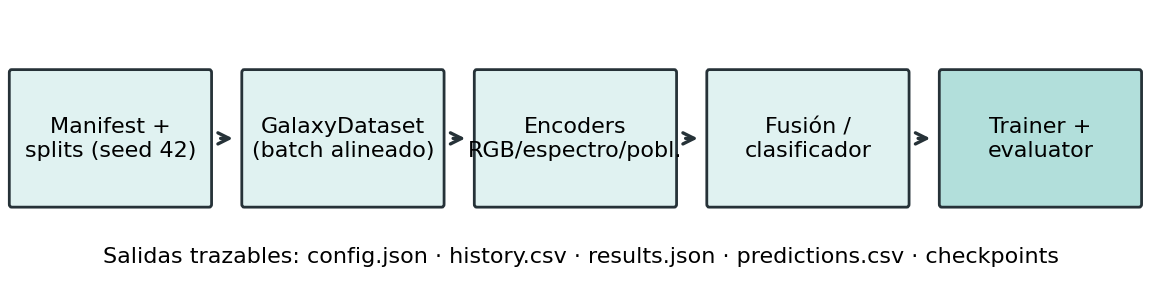
\includegraphics[width=0.95\textwidth]{figs/fig_pipeline.png}
\caption{Pipeline experimental modular. Cada corrida produce configuración, historial, resultados, predicciones por galaxia y checkpoints, lo que habilita el análisis de errores pareado de la Sección~\ref{sec:resultados}.}
\label{fig:pipeline}
\end{figure}

% =====================================================================
\section{Metodología y modelos}
\label{sec:metodologia}

\subsection{Protocolo común}
Todos los modelos se entrenaron con AdamW \citep{loshchilov2019}, pérdida \texttt{BCEWithLogitsLoss} y selección del checkpoint por AUC de validación; la evaluación se hizo en el mismo conjunto de prueba de 1,403 galaxias. La métrica primaria es ROC-AUC; la exactitud se reporta al umbral 0.5.

\subsection{Línea base y ablación (Avance 3)}
Se entrenaron encoders unimodales y combinaciones por concatenación:
\begin{itemize}
  \item \textbf{RGB}: una CNN compacta de 4 bloques y ResNet-18 \citep{he2016}.
  \item \textbf{Espectro observado}: CNN1D con \emph{pooling} global sobre \texttt{FLUX\_FoV}.
  \item \textbf{Espectro STARLIGHT}: CNN1D sobre el espectro sintético.
  \item \textbf{Poblaciones}: MLP sobre las $2\times45$ fracciones.
  \item \textbf{Combinaciones}: RGB + espectros, RGB + poblaciones y trimodal.
\end{itemize}
Se adoptó como \textbf{línea base visual} la ResNet-18 (AUC = 0.9633; exactitud = 88.8\,\%), por ser la arquitectura estándar de referencia en la literatura de morfología. La Tabla~\ref{tab:ablacion} muestra el resultado.

\begin{table}[htbp]
\centering
\caption{Ablación en el conjunto de prueba ($n=1{,}403$). Exactitud al umbral 0.5.}
\label{tab:ablacion}
\small
\begin{tabular}{llcc}
\toprule
\textbf{Modalidad} & \textbf{Modelo} & \textbf{ROC-AUC} & \textbf{Exactitud}\\
\midrule
Imagen & CNN 4 bloques & 0.9623 & 90.1\,\%\\
Imagen & ResNet-18 (\textbf{línea base}) & 0.9633 & 88.8\,\%\\
Trimodal & RGB + espectro + poblaciones (concat.) & 0.9650 & 89.0\,\%\\
Poblaciones & MLP STARLIGHT & 0.8949 & 83.7\,\%\\
Espectro SL & CNN1D & 0.8642 & 78.9\,\%\\
Espectro FoV & CNN1D & 0.8572 & 79.5\,\%\\
\bottomrule
\end{tabular}
\end{table}

La mejor fusión supera a la ResNet-18 por solo $\Delta\text{AUC}=+0.0017$, inferior a la incertidumbre del AUC ($\approx 0.005$): la mejora \emph{no está demostrada}. El diagnóstico de curvas de aprendizaje reveló patrones distintos por modalidad (Tabla~\ref{tab:diagnostico}): la imagen sobreajusta y el espectro subajusta. Por lo tanto, entrenar más no era la solución; había que cambiar la representación espectral.

\begin{table}[htbp]
\centering
\caption{Diagnóstico de generalización (pérdida final de entrenamiento / validación).}
\label{tab:diagnostico}
\small
\begin{tabularx}{\textwidth}{lcY}
\toprule
\textbf{Modelo} & \textbf{Train / Val} & \textbf{Lectura}\\
\midrule
CNN visual compacta & 0.237 / 0.287 & Sobreajuste leve tras la época 38; extender a 46 épocas no mejoró la prueba\\
ResNet-18 visual & 0.159 / 0.317 & Sobreajuste claro; también presente en las fusiones\\
CNN1D espectral & 0.461 / 0.475 & Subajuste / meseta: problema de representación y optimización\\
\bottomrule
\end{tabularx}
\end{table}

\subsection{Modelos candidatos: rediseño del experto espectral (Avance 4)}
La hipótesis fue que el \emph{pooling} global de la CNN1D destruía las relaciones entre el continuo, el quiebre de 4000\,\AA{} y las líneas. Se probaron tres variantes, todas con tasa de aprendizaje $3\times10^{-4}$, recorte de gradiente 1.0 y mayor capacidad: (i) CNN profunda con \emph{attention pooling} sin recurrencia (control), (ii) CNN + BiGRU \citep{cho2014} sobre 256 tokens y (iii) \emph{Patch} + BiGRU (128 parches de 32 puntos, BiGRU de 2 capas).

\begin{figure}[htbp]
\centering
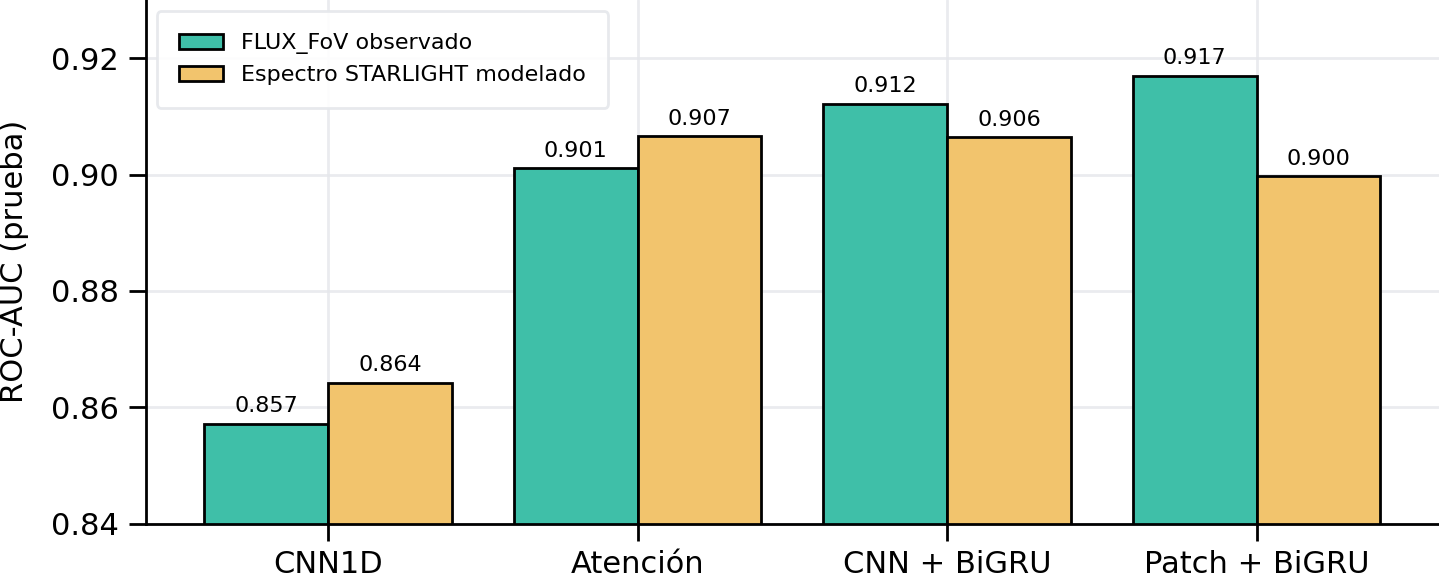
\includegraphics[width=0.9\textwidth]{figs/fig_espectros.png}
\caption{ROC-AUC en prueba de los encoders espectrales. El rediseño eleva el espectro observado de 0.857 a 0.917 (exactitud de 79.5\,\% a 85.2\,\%).}
\label{fig:espectros}
\end{figure}

El espectro sí contenía más señal (Figura~\ref{fig:espectros}): el mejor encoder FoV (Patch + BiGRU) alcanzó AUC = 0.9170 y exactitud = 85.2\,\%. El control con atención, sin recurrencia, ya llega a 0.9011 (FoV) y 0.9066 (STARLIGHT), por lo que la ganancia \emph{no} puede atribuirse solo a la BiGRU: optimización y encoder cambiaron a la vez.

\subsection{Selección del modelo final (Avance 5)}
\paragraph{Un experto espectral más fuerte no garantizó una mejor fusión.} Al concatenar la imagen con el encoder de atención sobre STARLIGHT, el AUC cayó de 0.9667 (imagen sola, mismo control de LR $3\times10^{-4}$) a 0.9334 ($-0.0333$); la fusión alcanzó su mejor checkpoint en la época 4 de 12, un síntoma compatible con atajos o memorización de la rama nueva. Es una sola corrida con una semilla: evidencia sugestiva, no prueba general.

\paragraph{La fusión tardía tampoco mejoró.} Promediar probabilidades RGB y de poblaciones con un peso global $\alpha$ fijo produjo $\Delta\text{AUC}=+0.0005$ con IC\,95\,\% $[-0.0012,\,+0.0022]$, que incluye el cero.

\paragraph{La decisión que importó.} Se eligió como \textbf{modelo final} la \textbf{CNN visual entrenada con LR $3\times10^{-4}$} (AUC = 0.9667; exactitud = 89.5\,\%), y se descartó la fusión por concatenación como modelo de producción. El porqué es triple: (1) ninguna fusión mostró una ganancia estadísticamente defendible; (2) la fusión añade costo de inferencia y una dependencia del espectro que LSST no podrá satisfacer a escala; y (3) el análisis de errores (Sección~\ref{sec:resultados}) reveló que la información complementaria existe, pero que la concatenación no es el mecanismo adecuado para explotarla. Esta decisión convierte un resultado aparentemente negativo (``la fusión no ayuda'') en una hipótesis más precisa para el trabajo futuro.

\begin{figure}[htbp]
\centering
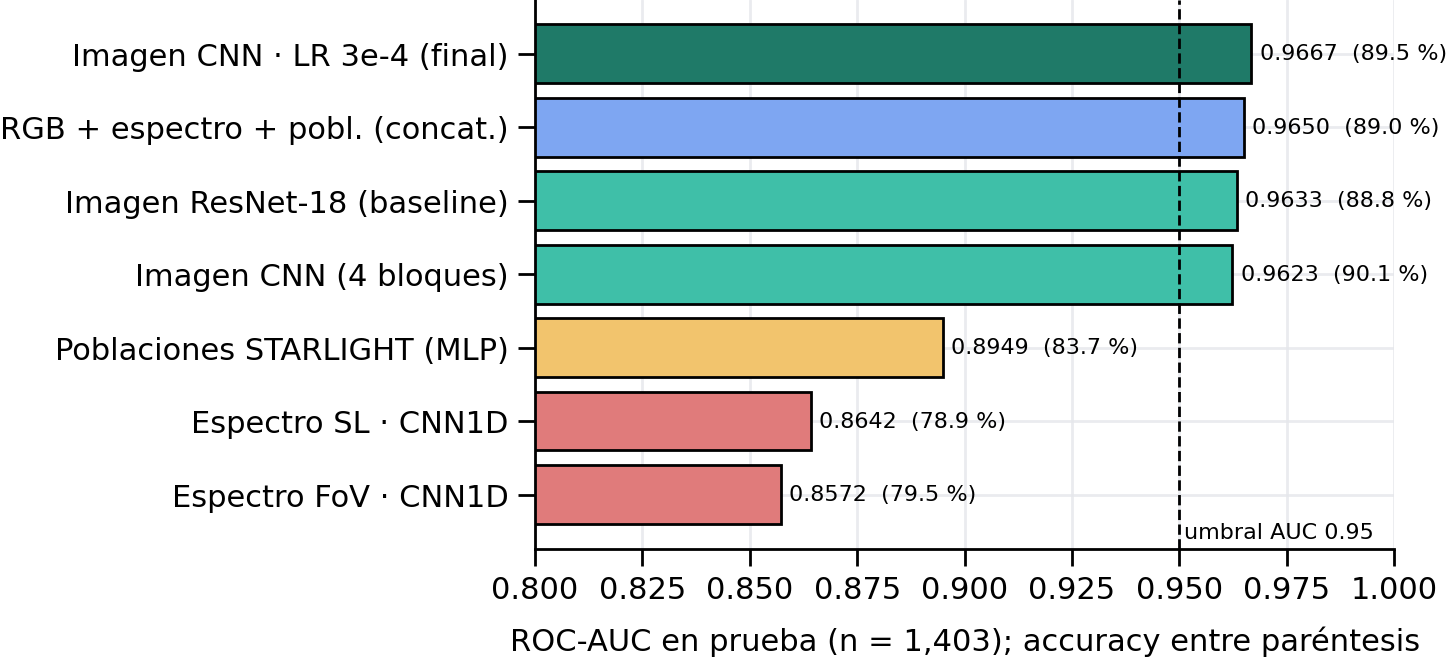
\includegraphics[width=0.95\textwidth]{figs/fig_ablacion.png}
\caption{Trayectoria de modelos: espectrales, de poblaciones, visuales y fusión. La línea discontinua marca el umbral de aceptación ROC-AUC $=0.95$.}
\label{fig:ablacion}
\end{figure}

% =====================================================================
\section{Resultados y validación}
\label{sec:resultados}

\subsection{Modelo final frente a línea base y umbrales}
La Tabla~\ref{tab:veredicto} contrasta el modelo final con la línea base y con los criterios de la Tabla~\ref{tab:criterios}.

\begin{table}[htbp]
\centering
\caption{Veredicto frente a los umbrales del proyecto. Brecha = observado $-$ umbral.}
\label{tab:veredicto}
\small
\begin{tabularx}{\textwidth}{p{3.9cm}p{1.4cm}p{3.6cm}Y}
\toprule
\textbf{Criterio} & \textbf{Umbral} & \textbf{Observado} & \textbf{Brecha / estado}\\
\midrule
ROC-AUC (métrica primaria) & $\geq 0.95$ & 0.9667 & $+0.0167$ · \textbf{cumple}\\
Lift vs.\ línea base ResNet-18 (0.9633) & --- & $+0.0034$ AUC; $+0.7$ pp exactitud & Menor que la incertidumbre ($\approx0.005$): no significativo\\
Lift vs.\ clasificador trivial & --- & $+0.4667$ AUC; $+27.1$ pp exactitud & Frente a AUC 0.5 y exactitud 62.4\,\%\\
Exactitud balanceada & $\geq 0.90$ & No reportada & Pendiente; la exactitud global (89.5\,\%) queda $-0.5$ pp bajo 0.90\\
Calibración (ECE) & $\leq 0.05$ & No medida & Pendiente\\
Mejora multimodal (IC\,95\,\% excluye 0) & IC $>0$ & $+0.0005$ $[-0.0012,+0.0022]$ & \textbf{No cumple}\\
\bottomrule
\end{tabularx}
\end{table}

El veredicto es mixto y debe leerse con honestidad: el sistema \emph{cumple} la métrica primaria con margen, pero \emph{no demuestra} la hipótesis multimodal y aún no tiene evidencia de calibración ni de exactitud balanceada. Además, la diferencia entre el modelo final y la línea base es menor que la incertidumbre del AUC; en la práctica, ambos son clasificadores visuales equivalentes, y la elección del final se justifica por su mayor AUC y su menor costo, no por una superioridad demostrada.

\subsection{Complementariedad: los errores no son idénticos}
El análisis pareado por galaxia sobre las mismas 1,403 observaciones de prueba mostró que:
\begin{itemize}
  \item la ResNet-18 visual comete \textbf{157 errores} (exactitud 88.8\,\%);
  \item el experto de poblaciones acierta el \textbf{51.6\,\%} de ellos; 76 errores son compartidos por ambos modelos;
  \item un oráculo que eligiera siempre el modelo correcto elevaría la exactitud de 0.888 a \textbf{0.946}.
\end{itemize}
El oráculo usa la etiqueta de forma retrospectiva: demuestra \emph{potencial}, no un clasificador realizable. Su valor es acotar el beneficio máximo que un decisor adaptativo podría capturar.

\subsection{Dónde se equivoca el modelo: la frontera morfológica}
La dificultad se concentra en la frontera Ttype 0--1 (Figura~\ref{fig:frontera}): estas galaxias son el 16.1\,\% de la muestra, pero concentran el \textbf{47.8\,\%} de los errores RGB, con una tasa de error de \textbf{33.2\,\%}. Fuera de esa frontera, el error visual es de solo \textbf{7.0\,\%}. Ninguna propiedad STARLIGHT individual separó significativamente los errores tras la corrección de Bonferroni, y la presencia de errores de alta confianza impide una regla simple basada solo en la incertidumbre.

\begin{figure}[htbp]
\centering
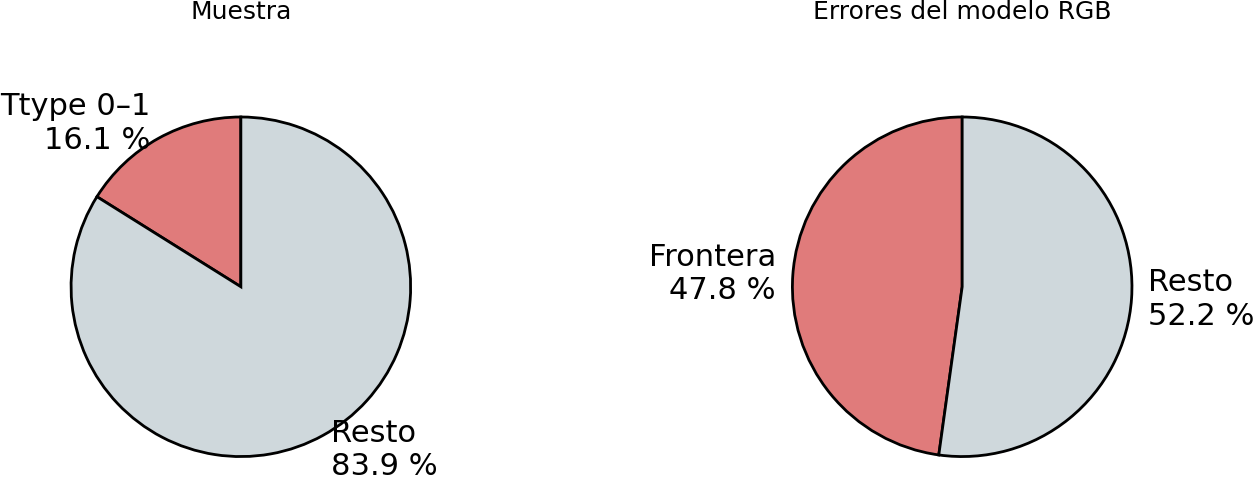
\includegraphics[width=0.85\textwidth]{figs/fig_frontera.png}
\caption{Concentración de errores. La frontera Ttype 0--1 es una minoría de la muestra, pero aporta casi la mitad de los errores del modelo visual.}
\label{fig:frontera}
\end{figure}

\subsection{Significado de los errores en el contexto del negocio}
Un error no tiene el mismo costo científico en todas partes:
\begin{itemize}
  \item \textbf{En la frontera (S0 frente a espirales tempranas)}, la propia etiqueta es ruidosa: la dispersión entre clasificadores humanos es máxima. Una discrepancia allí no necesariamente es un fallo del modelo; a menudo refleja una ambigüedad física real. Para el usuario, la acción correcta es \emph{derivar a revisión} o reportar la probabilidad, no forzar una etiqueta.
  \item \textbf{Fuera de la frontera}, un error del 7.0\,\% sí es relevante: una espiral clasificada como temprana sesga fracciones morfológicas, relaciones masa-morfología y estudios de apagado de la formación estelar. Estos errores son los que justifican el monitoreo y la calibración.
  \item \textbf{En términos económicos}, la concentración de errores sugiere una política de cobertura: clasificar automáticamente las galaxias con probabilidad extrema y enviar a revisión experta una fracción pequeña, enriquecida en Ttype 0--1. La curva cobertura-precisión que fija ese corte aún debe medirse.
\end{itemize}

\subsection{Limitaciones de validez integradas al resultado}
\begin{itemize}
  \item \textbf{Validez de etiquetas.} Ttype es un juicio humano; el techo alcanzable está limitado por el ruido en los tipos intermedios.
  \item \textbf{Contaminación entre modalidades.} STARLIGHT se deriva del mismo \texttt{FLUX\_FoV}; espectro y poblaciones no son evidencia independiente.
  \item \textbf{Una semilla por experimento.} Las diferencias de milésimas de AUC no son robustas sin 3--5 semillas e intervalos pareados.
  \item \textbf{Confusión de factores.} En los encoders espectrales cambiaron a la vez la tasa de aprendizaje y la arquitectura.
  \item \textbf{Reutilización del conjunto de prueba.} Comparar muchas variantes contra el mismo test introduce un sesgo optimista de selección; la estimación final requiere un conjunto ciego no consultado.
  \item \textbf{Supuesto de transferencia.} Los resultados se obtienen en galaxias cercanas de MaNGA; la profundidad, el \emph{seeing} y el corrimiento al rojo de LSST pueden degradar el desempeño.
\end{itemize}

% =====================================================================
\section{Implementación y operación}
\label{sec:implementacion}

Aunque el despliegue quedó fuera del alcance académico, CRISP-ML(Q) exige anticipar sus requisitos \citep{studer2021}. Se propone una arquitectura centrada en el clasificador visual, con revisión experta en la zona incierta.

\subsection{Requisitos para producción y responsables sugeridos}

\begin{table}[htbp]
\centering
\caption{Requisitos de operación y responsables sugeridos.}
\label{tab:requisitos}
\small
\begin{tabularx}{\textwidth}{p{3.6cm}Yp{3.2cm}}
\toprule
\textbf{Requisito} & \textbf{Detalle} & \textbf{Responsable sugerido}\\
\midrule
Ingesta y recorte & Descarga $g,r,z$; FOV $=k\cdot$\texttt{PETRO\_TH90}; $256\times256$; control de calidad e índices & Ingeniería de datos\\
Versionado de datos y modelo & Manifest, split, checksums, \texttt{config.json} y \emph{model card} en un registro de modelos & Ingeniería de ML (MLOps)\\
Calibración & Ajuste de temperatura o isotónico en validación; ECE $\leq 0.05$ antes de promover & Ciencia de datos\\
Política de decisión & Umbrales de probabilidad para auto-clasificar y para derivar a revisión; curva cobertura-precisión & Responsable del proyecto + experto de dominio\\
Revisión experta & Cola priorizada (Ttype 0--1 probable, baja confianza); etiquetas nuevas versionadas & Experto de dominio (astrónomo/a)\\
Infraestructura de inferencia & Contenedor reproducible, inferencia por lotes en GPU/CPU, registro de latencia y costo & Ingeniería de plataforma\\
Monitoreo y alertas & Tablero de deriva y desempeño; umbrales de alerta & MLOps + ciencia de datos\\
Reentrenamiento & Pipeline reproducible, mismo protocolo de split, test bloqueado, comparación contra el modelo vigente & Ingeniería de ML\\
Gobernanza & Aprobación de cada versión; trazabilidad modelo-catálogo & Responsable del proyecto\\
\bottomrule
\end{tabularx}
\end{table}

\subsection{Arquitectura de despliegue}
La Figura~\ref{fig:despliegue} muestra el flujo: las imágenes se ingieren y recortan con el mismo procedimiento del entrenamiento; el servicio de inferencia carga una versión registrada del modelo y produce $P(\text{tardía})$ calibrada; una política de decisión publica en el catálogo los casos de alta confianza y envía la zona incierta a revisión experta, cuyas etiquetas alimentan el reentrenamiento controlado.

\begin{figure}[htbp]
\centering
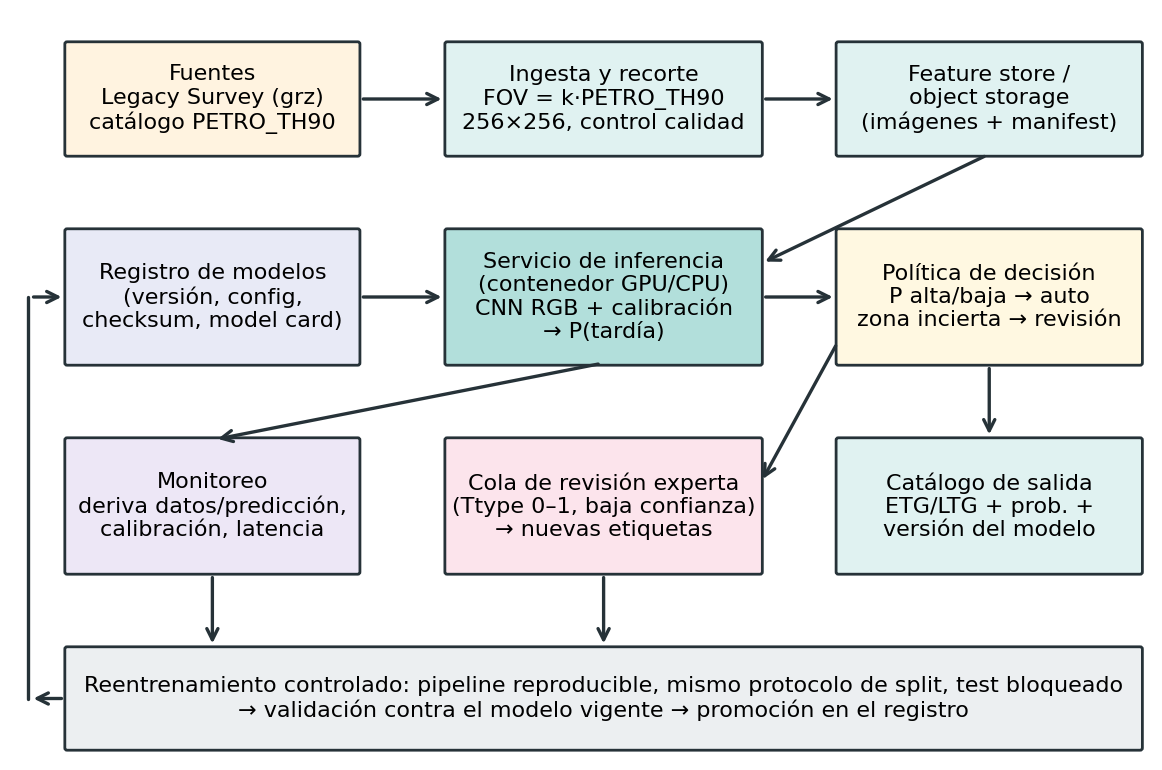
\includegraphics[width=0.92\textwidth]{figs/fig_despliegue.png}
\caption{Arquitectura de despliegue propuesta para el clasificador visual con revisión humana en la zona incierta y ciclo de reentrenamiento controlado.}
\label{fig:despliegue}
\end{figure}

El diseño es modular: si en el futuro se valida un decisor adaptativo, el experto espectral se añadiría como servicio opcional, invocado solo para galaxias con espectro y en la zona incierta, sin alterar la ruta principal.

\subsection{Monitoreo}

\begin{table}[htbp]
\centering
\caption{Aspectos a supervisar durante la operación.}
\label{tab:monitoreo}
\small
\begin{tabularx}{\textwidth}{p{3.3cm}Yp{3.6cm}}
\toprule
\textbf{Aspecto} & \textbf{Indicador} & \textbf{Acción ante alerta}\\
\midrule
Deriva de datos & Distribución de \texttt{PETRO\_TH90}, brillo, color y profundidad; región norte/sur del Legacy Survey & Revisar recorte; evaluar por subgrupo\\
Deriva de predicción & Fracción predicha de tardías frente al 62\,\% esperado; histograma de probabilidades & Auditoría de muestra\\
Calibración & ECE y Brier sobre las etiquetas de revisión experta & Recalibrar\\
Desempeño por segmento & AUC y error en Ttype 0--1, galaxias de canto y pequeñas & Reentrenar o ajustar la política\\
Cobertura & \% auto-clasificado con precisión $\geq 95\,\%$; volumen de la cola de revisión & Ajustar umbrales\\
Calidad de entrada & Recortes vacíos, estrellas superpuestas, artefactos & Filtrar en la ingesta\\
Operación & Latencia, galaxias/hora-GPU, costo, fallos & Escalar infraestructura\\
Explicabilidad & Muestreo periódico de mapas Grad-CAM \citep{selvaraju2017} & Detectar atajos (``Clever Hans'')\\
\bottomrule
\end{tabularx}
\end{table}

% =====================================================================
\section{Conclusiones clave}
\label{sec:conclusiones}

\subsection{Hallazgos principales}
\begin{enumerate}
  \item \textbf{La imagen es la referencia difícil de superar.} El modelo final visual alcanza ROC-AUC = 0.9667 y exactitud = 89.5\,\%, por encima del umbral de 0.95 (+0.0167). Su ventaja sobre la línea base ResNet-18 (+0.0034) no es significativa.
  \item \textbf{La hipótesis multimodal, tal como se formuló, no se confirmó.} Ninguna fusión mostró una mejora con un IC\,95\,\% que excluya el cero; la concatenación con un experto espectral más fuerte incluso degradó el AUC en 0.0333.
  \item \textbf{El espectro no era débil por falta de información.} Rediseñar el encoder elevó el AUC espectral de 0.857 a 0.917.
  \item \textbf{La complementariedad existe, pero no está explotada.} Las poblaciones corrigen el 51.6\,\% de los errores visuales; el oráculo acota el potencial en una exactitud de 0.946.
  \item \textbf{El error se concentra en la frontera física.} El 47.8\,\% de los errores ocurre en Ttype 0--1, donde la etiqueta es más ambigua.
\end{enumerate}

\subsection{Limitaciones}
Las conclusiones descansan en corridas de una sola semilla, en un conjunto de prueba reutilizado durante la selección, en etiquetas humanas ruidosas en la frontera y en dos ``modalidades'' espectrales que no son independientes. No se midieron la calibración, la exactitud balanceada ni la curva cobertura-precisión, de modo que el cumplimiento de los criterios económicos sigue abierto. Finalmente, el desempeño en galaxias cercanas de MaNGA no garantiza la transferencia a LSST.

\subsection{Trabajo futuro}
\begin{enumerate}
  \item \textbf{Reproducibilidad}: 3--5 semillas, intervalos pareados por bootstrap y prueba de McNemar \citep{dietterich1998}, reportando AUC y exactitud balanceada.
  \item \textbf{Calibración y análisis de errores}: ECE/Brier, diagramas de confiabilidad \citep{guo2017} y subgrupos por Ttype y masa.
  \item \textbf{Decisor adaptativo por galaxia}: $p_{\text{final}} = \alpha(x)\,p_{\text{RGB}} + [1-\alpha(x)]\,p_{\text{experto}}$, aprendido solo con predicciones fuera de pliegue (\emph{out-of-fold}) en entrenamiento y validación, con el test bloqueado; comparar fusión ponderada, \emph{stacking} y un \emph{gating} pequeño.
  \item \textbf{Destilación para LSST}: transferir lo aprendido por un modelo multimodal ``maestro'' a un estudiante solo-imagen, útil cuando no haya espectro.
  \item \textbf{Robustez}: ruido y PSF degradada, variación del factor de encuadre $\pm20\,\%$, invariancia a rotaciones y enmascaramiento de ventanas espectrales (H$\alpha$, quiebre de 4000\,\AA).
  \item \textbf{Etiquetas}: tratar la frontera Ttype 0--1 como clase de incertidumbre o usar etiquetas blandas a partir de la dispersión entre clasificadores \citep{walmsley2022}.
\end{enumerate}

% =====================================================================
\section{Referencias y anexos}
\label{sec:referencias}

\renewcommand{\refname}{}
\vspace{-2em}
\begin{thebibliography}{99}
\setlength{\itemsep}{2pt}\small

\bibitem[Bundy et~al.(2015)]{bundy2015}
Bundy, K., Bershady, M.~A., Law, D.~R., et~al. (2015). Overview of the SDSS-IV MaNGA survey: Mapping nearby galaxies at Apache Point Observatory. \emph{The Astrophysical Journal}, \emph{798}(1), 7. \url{https://doi.org/10.1088/0004-637X/798/1/7}

\bibitem[Buta(2013)]{buta2013}
Buta, R.~J. (2013). Galaxy morphology. En T.~D. Oswalt \& W.~C. Keel (Eds.), \emph{Planets, stars and stellar systems} (Vol.~6, pp.~1--89). Springer. \url{https://doi.org/10.1007/978-94-007-5609-0_1}

\bibitem[Cho et~al.(2014)]{cho2014}
Cho, K., van Merriënboer, B., Gulcehre, C., et~al. (2014). Learning phrase representations using RNN encoder--decoder for statistical machine translation. En \emph{Proceedings of EMNLP 2014} (pp.~1724--1734). \url{https://doi.org/10.3115/v1/D14-1179}

\bibitem[Cid Fernandes et~al.(2005)]{cidfernandes2005}
Cid Fernandes, R., Mateus, A., Sodré, L., Stasińska, G., \& Gomes, J.~M. (2005). Semi-empirical analysis of Sloan Digital Sky Survey galaxies -- I. Spectral synthesis method. \emph{Monthly Notices of the Royal Astronomical Society}, \emph{358}(2), 363--378. \url{https://doi.org/10.1111/j.1365-2966.2005.08752.x}

\bibitem[Dey et~al.(2019)]{dey2019}
Dey, A., Schlegel, D.~J., Lang, D., et~al. (2019). Overview of the DESI Legacy Imaging Surveys. \emph{The Astronomical Journal}, \emph{157}(5), 168. \url{https://doi.org/10.3847/1538-3881/ab089d}

\bibitem[Dietterich(1998)]{dietterich1998}
Dietterich, T.~G. (1998). Approximate statistical tests for comparing supervised classification learning algorithms. \emph{Neural Computation}, \emph{10}(7), 1895--1923. \url{https://doi.org/10.1162/089976698300017197}

\bibitem[Guo et~al.(2017)]{guo2017}
Guo, C., Pleiss, G., Sun, Y., \& Weinberger, K.~Q. (2017). On calibration of modern neural networks. En \emph{Proceedings of the 34th International Conference on Machine Learning} (pp.~1321--1330). PMLR.

\bibitem[He et~al.(2016)]{he2016}
He, K., Zhang, X., Ren, S., \& Sun, J. (2016). Deep residual learning for image recognition. En \emph{Proceedings of the IEEE Conference on Computer Vision and Pattern Recognition} (pp.~770--778). \url{https://doi.org/10.1109/CVPR.2016.90}

\bibitem[Hubble(1926)]{hubble1926}
Hubble, E.~P. (1926). Extragalactic nebulae. \emph{The Astrophysical Journal}, \emph{64}, 321--369. \url{https://doi.org/10.1086/143018}

\bibitem[Ivezić et~al.(2019)]{ivezic2019}
Ivezić, Ž., Kahn, S.~M., Tyson, J.~A., et~al. (2019). LSST: From science drivers to reference design and anticipated data products. \emph{The Astrophysical Journal}, \emph{873}(2), 111. \url{https://doi.org/10.3847/1538-4357/ab042c}

\bibitem[Loshchilov \& Hutter(2019)]{loshchilov2019}
Loshchilov, I., \& Hutter, F. (2019). Decoupled weight decay regularization. En \emph{International Conference on Learning Representations (ICLR)}.

\bibitem[Nair \& Abraham(2010)]{nair2010}
Nair, P.~B., \& Abraham, R.~G. (2010). A catalog of detailed visual morphological classifications for 14,034 galaxies in the Sloan Digital Sky Survey. \emph{The Astrophysical Journal Supplement Series}, \emph{186}(2), 427--456. \url{https://doi.org/10.1088/0067-0049/186/2/427}

\bibitem[Selvaraju et~al.(2017)]{selvaraju2017}
Selvaraju, R.~R., Cogswell, M., Das, A., et~al. (2017). Grad-CAM: Visual explanations from deep networks via gradient-based localization. En \emph{Proceedings of the IEEE International Conference on Computer Vision} (pp.~618--626). \url{https://doi.org/10.1109/ICCV.2017.74}

\bibitem[Studer et~al.(2021)]{studer2021}
Studer, S., Bui, T.~B., Drescher, C., et~al. (2021). Towards CRISP-ML(Q): A machine learning process model with quality assurance methodology. \emph{Machine Learning and Knowledge Extraction}, \emph{3}(2), 392--413. \url{https://doi.org/10.3390/make3020020}

\bibitem[Vázquez-Mata et~al.(2022)]{vazquezmata2022}
Vázquez-Mata, J.~A., Hernández-Toledo, H.~M., Avila-Reese, V., et~al. (2022). SDSS IV MaNGA: Visual morphological and statistical characterization of the DR15 sample. \emph{Monthly Notices of the Royal Astronomical Society}, \emph{512}(2), 2222--2244. \url{https://doi.org/10.1093/mnras/stac635}

\bibitem[Walmsley et~al.(2022)]{walmsley2022}
Walmsley, M., Lintott, C., Géron, T., et~al. (2022). Galaxy Zoo DECaLS: Detailed visual morphology measurements from volunteers and deep learning for 314\,000 galaxies. \emph{Monthly Notices of the Royal Astronomical Society}, \emph{509}(3), 3966--3988. \url{https://doi.org/10.1093/mnras/stab2093}

\end{thebibliography}

\appendix
\renewcommand{\thesection}{\Alph{section}}
\section*{Anexo A. Glosario}
\addcontentsline{toc}{subsection}{Anexo A. Glosario}
\small
\begin{tabularx}{\textwidth}{lY}
\toprule
\textbf{Término} & \textbf{Definición}\\
\midrule
ETG / LTG & Galaxia temprana (elíptica o lenticular) / tardía (espiral o irregular)\\
Ttype & Codificación numérica de la secuencia de Hubble; $\leq0$ temprana, 1--10 tardía\\
\texttt{PETRO\_TH90} & Radio que encierra el 90\,\% de la luz petrosiana; controla el encuadre\\
\texttt{FLUX\_FoV} & Espectro integrado en todo el campo del IFU de MaNGA\\
STARLIGHT & Código de síntesis espectral que ajusta el espectro con 45 plantillas de poblaciones\\
ROC-AUC & Probabilidad de que el modelo ordene una tardía por encima de una temprana elegidas al azar\\
ECE & Error esperado de calibración: discrepancia entre la probabilidad predicha y la frecuencia observada\\
Oráculo & Selector ideal que elige el modelo correcto con conocimiento de la etiqueta (cota superior)\\
\bottomrule
\end{tabularx}
\normalsize

\section*{Anexo B. Trazabilidad de cifras y artefactos}
\addcontentsline{toc}{subsection}{Anexo B. Trazabilidad}
Todas las cifras del artículo provienen del informe integrado de avances (noviembre de 2026) y de los notebooks del repositorio del proyecto (\url{https://github.com/Melonangie/Galaxy-Vision}, carpetas \texttt{Notebooks/avances} y \texttt{Notebooks/julio}). Cada corrida conserva \texttt{config.json}, \texttt{history.csv}, \texttt{results.json}, \texttt{predictions.csv}, matrices de confusión y checkpoints. Los criterios de la Tabla~\ref{tab:criterios} provienen del documento de planeación CRISP-ML(Q) del proyecto.

\begin{table}[htbp]
\centering
\caption{Resumen de cifras decisivas.}
\label{tab:cifras}
\small
\begin{tabular}{lc}
\toprule
\textbf{Cifra} & \textbf{Valor}\\
\midrule
Cohorte alineada / manifest & 9,351 / 10,014\\
Clasificador trivial (exactitud; AUC) & 62.4\,\%; 0.500\\
Línea base ResNet-18 (AUC; exactitud; errores) & 0.9633; 88.8\,\%; 157\\
Modelo final CNN visual LR $3\times10^{-4}$ (AUC; exactitud) & 0.9667; 89.5\,\%\\
Lift final vs.\ línea base (AUC) & $+0.0034$\\
Brecha frente al umbral AUC 0.95 & $+0.0167$\\
Mejor encoder espectral (Patch + BiGRU, FoV) & 0.9170; 85.2\,\%\\
Fusión tardía $\Delta$AUC (IC\,95\,\%) & $+0.0005$ $[-0.0012,+0.0022]$\\
Concatenación con atención SL $\Delta$AUC & $-0.0333$\\
Errores RGB corregidos por poblaciones / oráculo & 51.6\,\% / 0.946\\
Frontera Ttype 0--1: muestra / errores / tasa & 16.1\,\% / 47.8\,\% / 33.2\,\%\\
\bottomrule
\end{tabular}
\end{table}

\end{document}
